%% IMPORTANT: Once working, run latex 3 times to get listoffigures to work

%% Be sure to check spelling!

%% Put **your** name and the proper due date in place

%% Copy the lstlisting and figure code as many times as you need
%% Be sure to put in your own file names if appropriate

%% Note that the \epsfig commands are currently commented out - until the
%%%% files exist, processing this code without them will result in an error
%%%% so leave the comments until you have created the graphics files!

\documentclass{article}
\usepackage{amsmath}    % loads AMS-Math package
\usepackage{epsfig}     % allows PostScript files
\usepackage{listings}   % allows lstlisting environment
\usepackage{moreverb}   % allows listinginput environment
\usepackage{vmargin}    % allows better margins
\setpapersize{USletter} % sets the paper size
\setmarginsrb{1in}{0.5in}{1in}{0.2in}{12pt}{11mm}{0pt}{11mm} %sets margins 
\begin{document}
\begin{center}
\rule{6.5in}{0.5mm}\\~\\
{\bf \large EGR 103L -- Fall 2016}\\~\\
{\huge \bf Laboratory 2 - Introduction to MATLAB}\\~\\
CEMAL YAGCIOGLU (cy111)\\
Lab Section 05, WEDNESDAY 11:45 AM - 2:35 PM\\
SEPTEMBER 18, 2016\\~\\
{\small I understand and have adhered to all the tenets of the Duke
  Community Standard in completing every part of this assignment.  I
  understand that a violation of any part of the Standard on any part
  of this assignment can result in failure of this assignment, failure
  of this course, and/or suspension from Duke University.} 
\rule{6.5in}{0.5mm}\\
\end{center}
\tableofcontents
\listoffigures
\pagebreak

\section{Introduction}
My Matlab program loads the data for Beam1, and copies each column into new variables. It converts the Mass(kg) data to Force(N) by multiplying it by 9.81(N/kg). It converts the Displacement data in inches to meters by multiplying it by (2.54/100). With polyfit command, it finds first order fit polynomials. Then it generates predictions by creating 100 representational Force values, and calculating Displacement predictions. It plots Displacement as a function of Force and the plot values on the same graph. Finally it labels graph with appropriate titles, and saves the graph. It goes through the same procedure to Beam2 and Beam3 data. We are expected to observe these three data to see which graph fits most to the Displacement as a function of Force graph to conclude which Beam acts like a spring(acts according to Hooke's Law). 

\section{Data Obtained}
The three data sets from the experiments are presented in Table
\ref{DataTables}.
% replace the tables below with *your* data sets.  You may cut and paste
% from the MATLAB window and then add \\ and & as needed

\renewcommand{\arraystretch}{1.4}
\begin{table}[h]
\begin{center}
\begin{tabular}{ccc}
\begin{tabular}[t]{|c|c|}\hline
\multicolumn{2}{|c|}{Beam1.dat}\\ \hline
{\bf Mass} & {\bf Disp.}\\
(kg) & (in)\\ \hline
0.0000000e+00&	1.0506442e-01\\
2.4969314e-01&	1.5393050e-01\\
4.9938629e-01&	9.1829900e-02\\
7.4907943e-01&	1.9121739e-01\\
9.9877258e-01&	3.3852003e-01\\
1.2484657e+00&	6.4140472e-01\\
1.4981589e+00&	1.1599771e+00\\
1.7478520e+00&	1.8051665e+00\\
1.9975452e+00&	2.6829435e+00\\
2.2472383e+00&	3.6913222e+00\\
2.4969314e+00&	5.1911317e+00\\
\hline
\end{tabular}
&
\begin{tabular}[t]{|c|c|}\hline
\multicolumn{2}{|c|}{Beam2.dat}\\ \hline
{\bf Mass} & {\bf Disp.}\\
(kg) & (in)\\ \hline
0.0000000e+00&	2.8577720e-03\\
2.4018292e-01&	7.7785719e-01\\
4.8036585e-01&	1.3496902e+00\\
7.2054877e-01&	1.6343995e+00\\
9.6073170e-01&	2.2155730e+00\\
1.2009146e+00&	2.6345051e+00\\
1.4410975e+00&	3.1922596e+00\\
1.6812805e+00&	3.5522297e+00\\
1.9214634e+00&	3.8456644e+00\\
2.1616463e+00&	4.6163926e+00\\
 \hline
\end{tabular}
&
\begin{tabular}[t]{|c|c|}\hline
\multicolumn{2}{|c|}{Beam3.dat}\\ \hline
{\bf Mass} & {\bf Disp.}\\
(kg) & (in)\\ \hline
0.0000000e+00&	2.5207794e-03\\
3.4636619e-02&	4.6555129e-02\\
6.9273237e-02&	8.9037799e-02\\
1.0390986e-01&	1.3197719e-01\\
1.3854647e-01&	1.7271271e-01\\
1.7318309e-01&	2.1775915e-01\\
2.0781971e-01&	2.4015748e-01\\
2.4245633e-01&	2.4015748e-01\\
2.7709295e-01&	2.4015748e-01\\
 \hline
\end{tabular}
\end{tabular}
\caption{Data from Three Beam Experiments \label{DataTables}}
\end{center}
\end{table}

\section{Calculation Results}
A first-order polynomial fitting algorithm determined that 
the coefficients given in Table \ref{Coefs} 
produce the best-fit of the data to a straight line.
% replace the Greek letters with your calculations

\begin{table}[h]
\begin{center}
\begin{tabular}{r|c|c}
Data File & Compliance (m/N) & Init. Disp. (m)\\ \hline \hline
{\tt Beam1.dat} & 4.8456e-03 & -2.2280e-02 \\ \hline
{\tt Beam2.dat} & 5.1680e-03 &  5.7105e-03 \\ \hline
{\tt Beam3.dat} & 2.3913e-03 &  6.4745e-04 \\ \hline
\end{tabular}
\caption{Table of Compliances and Initial Displacement Values \label{Coefs}}
\end{center}
\end{table}
\pagebreak % turn this on if it makes sense to do so by removing the first %

\section{Conclusions}
For all three data we obtained a graph, a compliance value and a initial displacement value. Compliance value and Initial Displacement value was used to graph of data according to Hooke's law. Data for Beam2 was the most fitting to its own Hooke's Law graph. Thus, Beam2 acted most like a usual spring. The other two did not match well to the equation that modeled the force displacement relationship, therefore Beam1 and Beam3 did not act like a spring.
\pagebreak

\appendix
\section{Codes}
% Put the name of your file in the subsection name 
% and the listinginput input; or use the names given below
% Be sure to include the community standard in codes!
% Add \pagebreaks if they make sense
\subsection{DoneBeam1.m}
\listinginput[1]{1}{DoneBeam1.m}
\pagebreak 
\subsection{DoneBeam2.m}
\listinginput[1]{1}{DoneBeam2.m}
\pagebreak 
\subsection{DoneBeam3.m}
\listinginput[1]{1}{DoneBeam3.m}
\pagebreak  % this will start figures on a new page 

\section{Figures}
%%% Almost everything in this section is done; make sure you 
%%% understand how it works in general and be sure to 
%%% uncomment the epsfig lines once you have created the graphs
\begin{figure}[htb]
\begin{center}
\epsfig{file=Beam1Plot.eps, width=3.5in}
\caption{Displacement vs. Force for Beam 1}
\end{center}
\end{figure}

\begin{figure}[htb]
\begin{center}
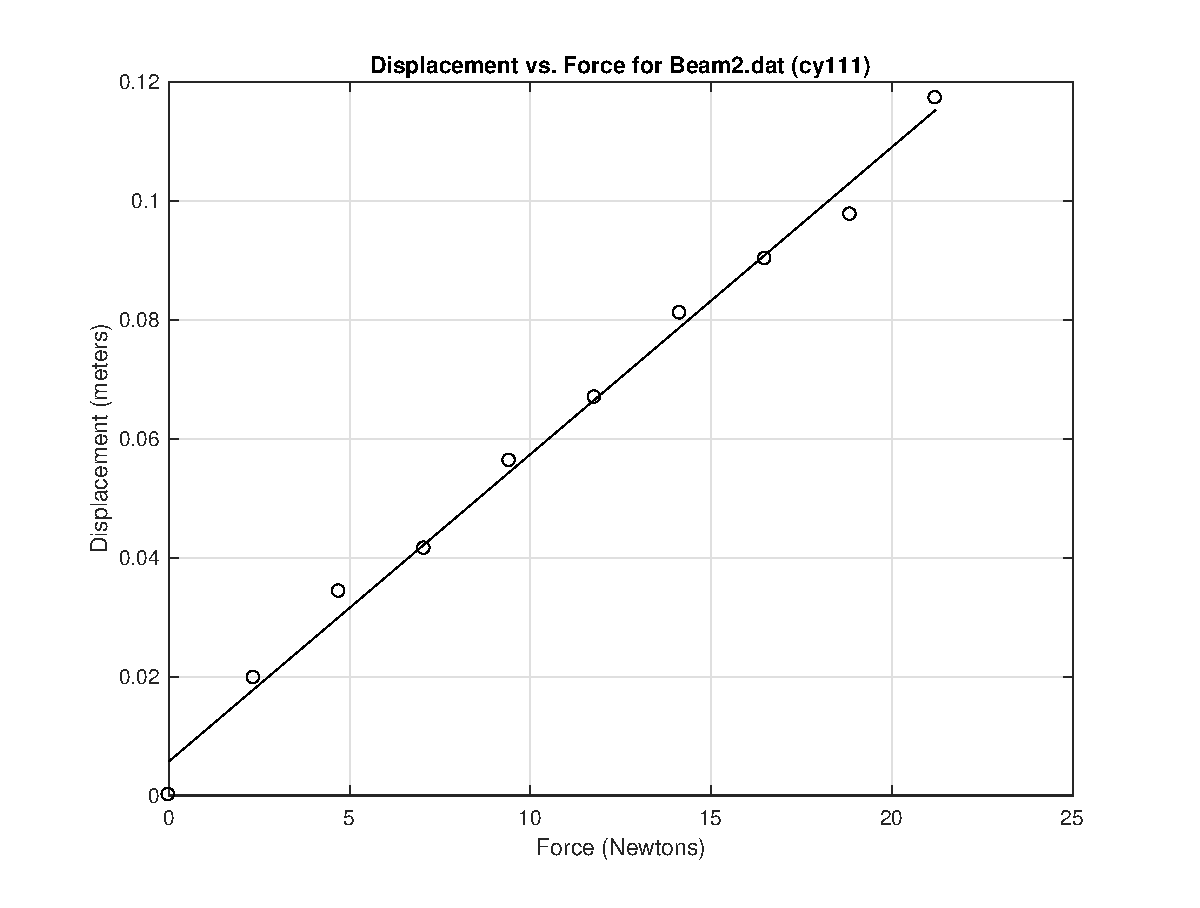
\epsfig{file=Beam2Plot.eps, width=3.5in}
\caption{Displacement vs. Force for Beam 2}
\end{center}
\end{figure}

\begin{figure}[htb]
\begin{center}
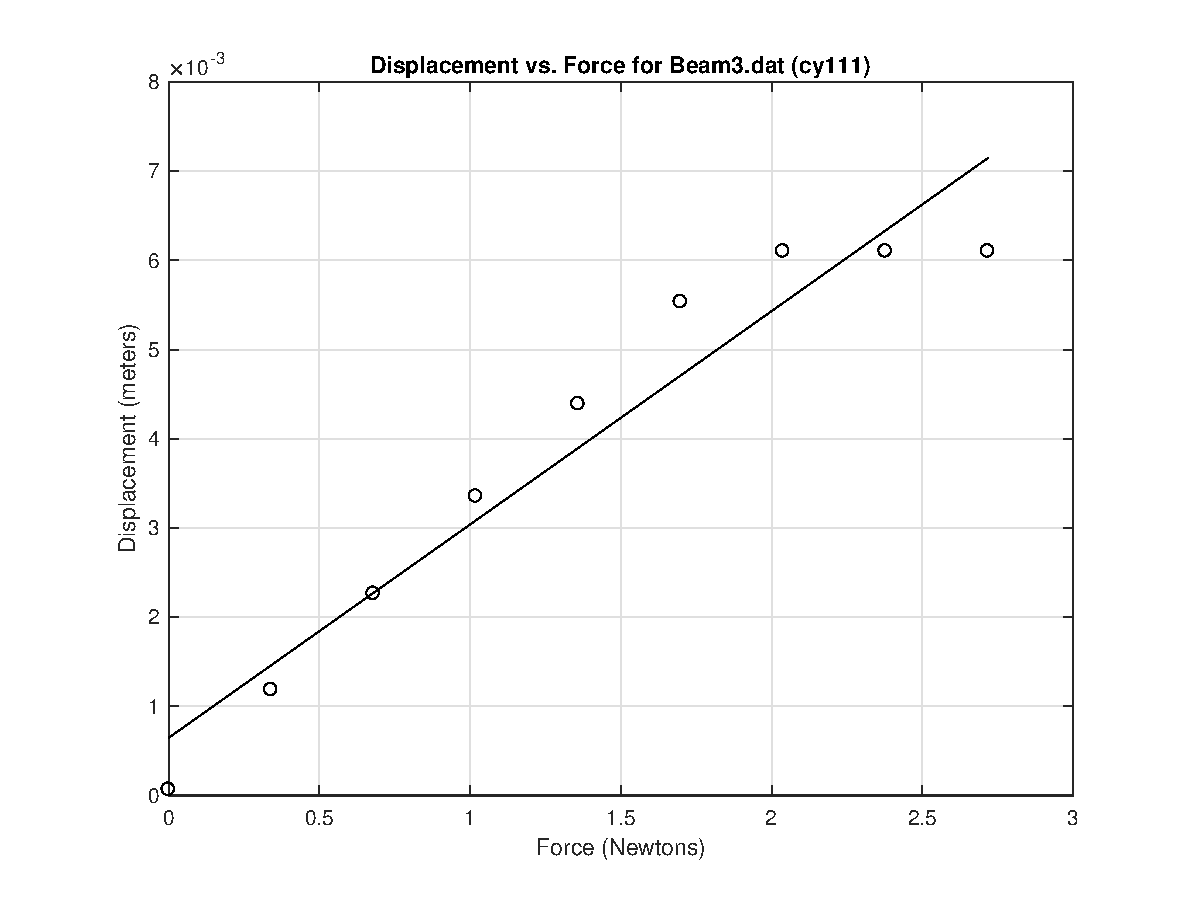
\epsfig{file=Beam3Plot.eps, width=3.5in}
\caption{Displacement vs. Force for Beam 3}
\end{center}
\end{figure}
\end{document}
